\documentclass[conference,compsoc,onecolumn]{IEEEtran}
\usepackage{graphicx}
\usepackage{multirow}
\usepackage{array}
\usepackage{listings}
\usepackage{xcolor}   % for \textcolor
\usepackage{amsmath}  % for \hookrightarrow
\usepackage{gensymb}

% Document Setup
\setlength\extrarowheight{2pt} % Space for tables
\lstset{
	literate={θ}{{$\theta$}}1
			 {δ}{{$\delta$}}1
			 {τ}{{$\tau$}}1
			 {λ}{{$\lambda$}}1
			 {η}{{$\eta$}}1
			 {μ}{{$\mu$}}1
			 {∈}{{$\in$}}1
			 {σ}{{$\sigma$}}1
			 {∞}{{$\infty$}}1
}

\lstset{
	frame=single,
	breaklines=true,
	postbreak=\mbox{\textcolor{red}{$\hookrightarrow$}\space},
}

\begin{document}

\title{SYSC5500F Project Report\\ Cell-DEVS Model of Bee Swarm Behaviour}

\author{
\IEEEauthorblockN{James Baak}
\IEEEauthorblockA{Department of Systems and Computer Engineering\\
Carleton University\\
Ottawa, Canada\\
Email: james.baak@carleton.ca}
}

\maketitle

\begin{abstract}
This project builds off the previous work of a bee cellular automata model with a dependency on temperature presented by M. Stefanec et al. in 2017 \cite{Stefanc2017}. Improvements are made in the design and implementation of the cellular automata by using Cell-DEVS to improve the simulation performance for further analysis. Changes to the cellular model are made to study the simple behaviour of the bees to examine how they cluster and if the temperature controlling robots can change the overall structure of the hive. Various simulations are run to attempt to understand the current cellular model of the bee's behaviour and how they interact in a closed environment in response to temperature.
\end{abstract}

\begin{IEEEkeywords}
	Cell-DEVS, Swarm, Bees, Thermal, Control
\end{IEEEkeywords}

\section{Introduction}

Complex natural systems can have simple underlying mechanisms that drive them to create interesting patterns. The simple underlying mechanisms of natural systems can be approximately modeled in order to study the natural world in simulations without affecting the natural world negativity. These models allow scientists to further study natural and biological systems which may be difficult to study otherwise. Using techniques like cellular automata to discretize space and allow the study of entities and other factors through time and record results that would be objectively much harder to obtain in the real world. A recent study and model of bees has been created in \cite{Stefanc2017, Szopek2017} to evaluate bees behaviour in groups with respect to local temperature. The researchers determined that a cellular model of bees can be developed to analysis their grouping behaviour in temperature controlled environments. This paper proposes to take another step into studying a bee's behaviour by slightly modifying the original model to study the grouping mechanics of bees on a 2D plane. Creating such a model would enable further research and experimentation into hive and insect structures and aid in our understanding of animals.

An introduction and explanation of the original cellular automata is described in section \ref{background} to provide the necessary information to understand the complete model definition in section \ref{model}. Section \ref{model} discusses the cellular model and changes made to it to be adapted to Cell-DEVS. This section also defines the formal Cell-DEVS specification and its implementation in CD++. Next, section \ref{results} defines some hypotheses and contains the results from the various simulations run and some discussion of the cellular model behaviour. Finally, the simulation results are discussed further in section \ref{conclusion} to analyze the performance and accuracy of the model and any improvements that could be made in future iterations of the project in developing a cellular model representation of an internal structure of a beehive or similar insects.

\section{Background}\label{background}

The basis for this research and project was founded by continuing the work in \cite{Stefanc2017, Szopek2017}. Stefanec et al. constructed and verified a cellular automata model for describing the behaviour of bees on a two dimensional (2D) plane reacting to changes in temperature. The model was developed by observing actual bees in a controlled environment. The bees shared the 2D plane with stationary Combined Actuator and Sensor Units (CASU) robots that could control the local robot's local temperature in its close surroundings and sense the bees. Figure \ref{figx1} shows some of the actual honeybees used in the experiments and a CASU robot. The goal of the original project was to attempt to determine whether the temperature feedback from the CASU robots could control the movement and clusters of the bees on the 2D plane. The project's results show that indeed the bees would cluster around the CASU robot outputting a higher temperature than the ambient temperature of the plane. The authors then developed a cellular automata model to emulate the real world bee behaviour with respect to their movement in regards to local temperature. The next few paragraphs will go into detail about their model and the different parameters needed to represent the behaviour of the bees.

\begin{figure}[htbp]
	\centerline{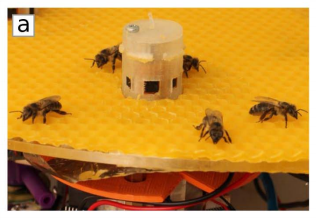
\includegraphics[scale=0.85]{../images/fig1a-stefanec2017.png}}
	\caption{Figure 1a from \cite{Stefanc2017}. The actual bees used for experimentation and verification of the cellular model. The stationary CASU robot can also be seen here.}
	\label{figx1}
\end{figure}

\subsection{Honeybee Behaviour}
The young honeybees in the cellular model can be represented by a series of parameters that determine their walking pattern, socialization, and their reaction to their local environment temperature \cite{Stefanc2017}. Every bee in the simulation will have the same parameters and can be varied at the start of the simulation to simulate different behaviours.

A random walking pattern is used for the bee's walking behaviour while it is not interacting with any other bees and traversing across the plane alone. The parameter $\alpha$ is dimensionless and used as the random walk parameter for the bee. It is set at 0.1 or 10\% and it used at each step of the bee to check whether the bee will turn or continue on its current path \cite{Stefanc2017}. Therefore, there is a 10\% chance for the bee to change its direction while it is walking.

In order for a bee to socialize, other bees must be present around the bee. The parameter $\sigma$, or known as the social factor, is a whole number that represents the number of cells to check around the bee in search for other bees to socialize with. The cells in the cellular model use a Moore neighborhood, meaning each cell will have 9 neighbors including itself. When a bee moves to a space, it searches $\sigma$ cells from its Moore neighborhood around it to determine if a bee is present. If a bee is present, then it may stop to socialize with the other bee(s). The $\sigma$ cells around the bee are chosen at random in \cite{Stefanc2017}. In \cite{Stefanc2017}, $\sigma$ was set to 3, so 3 random cells would be chosen at each cell in search for other bees to socialize with.

Once a bee or bees have been found to be in contact with a bee, there is a possibility of the bees to socialize. The parameter $\Psi$ represents the probability of a bee stopping and socializing with bees it is in contact with and called the stopping probability \cite{Stefanc2017}. In Stefanec et al. papers they use two different stopping probabilities. They started with 0.4 or a 40\% chance of socializing, but later increased the probability to 0.8, or 80\%, since it was determined to produce a more accurate result \cite{Stefanc2017}.

When two or more bees are within close proximity and start to socialize, they wait at their current cell for a period of time that is dependent on the current temperature of that cell. The waiting time in seconds can be calculated by the following equation presented in \cite{Stefanc2017}:

\begin{equation}
	f(T) = \frac{(a + b*T)^c}{(a + b*T)^c + d^c} * e + f
\end{equation}

where a = 3.09, b = -0.0403, c = -28.5, d = 1.79, e = 22.5, f = 0.645, and T is the temperature of a given cell. The function is one of sigmoid form that produces waiting times around 1 second for temperatures around 25 \degree C and 25 seconds for temperatures around 38 \degree C \cite{Stefanc2017}. From this equation, it can be extracted that the bees will wait or socialize for longer periods of time when the local environment is warmer.

The collection of the parameters described above enabled the simple representation of a bee's behaviour in a restricted environment with other factors of a bees life being removed, such as their chores to develop the hive and work with honey and larva. The bees were fed with honey before experimentation and bees that had visible deficiencies were not used in the original experiments \cite{Stefanc2017}.

\subsection{2D Arena}

The original area where the bees and CASU robots were placed were called the arena. In the experiments, the arena contained twelve bees and two CASU robots. The simulations used the same amount of bees and robots where each robot and bee took up exactly one cell. The simulated arena size was 7 by 14, so a total of 98 cells. Therefore, the approximate percentage of bee coverage is $(12 bee cells / 98 total cells) * 100 = 12.2 \% $. The percentage of bee coverage will be used later as a parameter for filling the arena with a proportional amount of bees to space for different arena sizes. 

\subsection{CASU Robots}

The goal of the two CASU robots is to provide positive feedback between the bees and the robots. The robot's temperature would change depending on the amount of the bees in its surroundings. The two CASUs on the arena also provide feedback to each other as when one CASU increases its temperature the other CASU's temperature would decrease \cite{Stefanc2017}. The ambient temperature of the environment was set to 28 \degree C using a heating pad, but the preferred temperature of young honeybees is around 36 \degree C, so the higher temperatures at the CASU robots would be preferred compared to a cooler CASU or ambient areas of the arena.

\subsection{Discrete Time Versus Discrete Event}

The original cellular automata that was developed for simulation in \cite{Stefanc2017} used a discrete time step approach in Python. Although Python is a very good language for visualization and has many open libraries, a discrete time step approach leads to the execution of every cell for each time step. Many of the cells in the simulation model would be blank and the checks could be avoided. Another issue of using discrete time steps is that the resolution of the simulation is limited by the precision of the each time step. To avoid this issue, one could use a discrete event approach to save on computational cycles while maintaining high precision by not limiting the resolution of the data. The goal of the following paper and project is to use Cell-DEVS which is an approach for formally constructing Discrete Event System Specifications (DEVS) for Cellular automata \cite{Wainer2009}.

\section{Cell-DEV Model for Bee Behaviour}\label{model}

A few changes were made to the original cellular model described above to allow for the implementation of the model in CD++ and for further exploration of bee swarm mechanics using the simple model presented in \cite{Stefanc2017, Szopek2017}. The bees were first implemented and tested on an unbounded 2D wrapped plane to allow the bees to quickly wrap around the plane without changing their random walk. The social factor, $\sigma$, selected three \emph{random} cells from a bee's neighborhood to determine whether it could socialize. As it would be difficult to choose three random unique cells in a bee's neighborhood, our Cell-DEVS model will check the three cells in front of the bee. Figure \ref{neighborhood} shows the neighborhood of a bee with each neighbors respective coded number to represent that space. For example, since our bee in figure \ref{neighborhood} is facing and traveling in the direction 2 (North), the social factor will check the three front cells. Therefore the cells 1 (North-west), 2 (North), and 3 (North-east) will be checked for bees.

\begin{figure}[htbp]
	\centerline{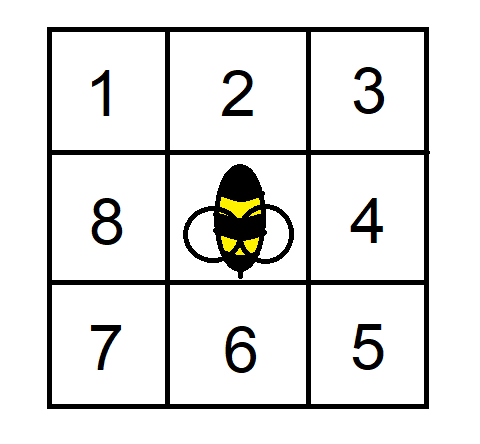
\includegraphics[scale=0.35]{../images/moore-neighbourhood.png}}
	\caption{The Moore neighborhood of a bee}
	\label{neighborhood}
\end{figure}

A larger change to the original model is that each bee will emit their own thermal energy and affect their surroundings. Before, the CASU robots were the only entities that could modify the local temperature, but now each bee will increase its neighborhood temperature by 1 \degree C. This enables the bees in the model to form their own clusters and favors socialization because as the bees cluster, the temperature of the cluster will increase making it more preferable than ambient space or being alone. Although this change hasn't been verified and tested, it is reasonable since the bees shouldn't only be attracted to the CASU robots as their only stimuli. With the bees affecting their local temperatures and thus the grouping and socializing behaviour of bees, it is hoped that the clusters formed in simulation will be similar to larger bee clusters in nature with and without the CASU robots.

\subsection{Model Definition}\label{def}

The following section describes the model definition and provides a description of each key component and entity in the system and their interactions. The model can be broken into several rules that guide each cell to behave how it should. The two active entities of the system are the blank cells and the bee cells because a blank cell is able to hold a bee and a bee cell is able to become a blank cell by moving into a blank cell.
\\
\\
There are four different entities a cell can be during a simulation:
\begin{enumerate}
	\item \emph{Blank Cell}: A cell representing empty space that a bee can move into
	\item \emph{Bee Cell}: A bee traveling or waiting in a cell space for a period of time
	\item \emph{Wall}: A stationary obstacle which bees can not move into
	\item \emph{CASU Robot}: A stationary obstacle that affects the temperature of surrounding cells
\end{enumerate}

To understand the model and how it is constructed, the state of each cell is described in detail here. Each cell holds multiple variables in its state so the cellular model can function properly. The variables of a cells state are encoded using integer shifting operations to encode all variables into a single state integer. The single state integer will always be four digits long due to the restricts of each variable. Variables can be extracted from the state integer by using unshift operations for use in functions and cell calculations. Each variable is described in table \ref{table:per}.

\begin{center}
	\begin{table*}[btp]
		\centering
		\caption{\\The variables used in the overall state of each cell}
		\begin{tabular}{ |c|c|c|c|c|  }
			\hline
			Entity Type & Variable & min & max & Description \\
			\hline
			\hline
			\multirow{3}{4em}{Blank Cell} & Temperature & 28 & 99 & The temperature of the cell \\ 
			& Move here & 0 & 8 & The number of bees with move intents here \\
			& Direction & 0 & 0 & The direction variable is 0 for blank cells \\
			\hline
			\multirow{3}{4em}{Bee Cell} & Temperature & 28 & 99 & The temperature of the cell \\ 
			& Move & 0 & 4 & The variable used to keep track of a bee's internal state \\
			& Direction & 1 & 8 & The direction that the bee is facing. Figure \ref{neighborhood} \\
			\hline
			\multirow{3}{4em}{Wall Cell} & Temperature & 28 & 99 & The temperature of the cell \\ 
			& Move & 0 & 0 & The move variable will be 0 for walls \\
			& Direction & 9 & 9 & The direction variable is 9 for wall and CASU cells \\
			\hline
			\multirow{3}{4em}{CASU Cell} & Temperature & 28 & 99 & The temperature of the cell \\ 
			& Move & 0 & 9 & The amount to raise the temperature by in the CASU's neighborhood \\
			& Direction & 9 & 9 & The direction variable is 9 for wall and CASU cells \\
			\hline
		\end{tabular}
		\label{table:per}
	\end{table*}
\end{center}

Table \ref{table:per} shows that each cell will have three variables to determine its state. Each cell entity type variables can be encoded as a single integer that represents its state. The following equations show the functions to encode and decode a cell's state:

\begin{equation}
	encode(T,M,D) = (T * 100) + (M * 10) + D
\end{equation}
\begin{equation}
	decode_T(state) = truncate(state / 100)
\end{equation}
\begin{equation}
	decode_M(state) = truncate(remainder(state,100) / 10)
\end{equation}
\begin{equation}
	decode_D(state) = remainder(remainder(state,100),10)
\end{equation}

where T is the temperature of a cell, M is the movement variable, and D is the direction variable. The encoded value in other word will represent a 4 digit number structured as TTMD. The encoded state can then be broken into its variables by using their respective decode function. The temperature of a cell can be determined by examining each of its neighbors. If a neighbor is another bee, then the temperature of the cell will increase by one. If a neighbor is a CASU robot, then the temperature of the cell will increase by the move variable of the CASU cell, as shown in table \ref{table:per}. Each addition will be added to the ambient temperature (28 \degree C) of the cell.
The parameters presented in section \ref{background} were left the same and are summarized in table \ref{table:sum}.

As described in table \ref{table:per}, the bee's Move variable is used to keep track of its internal state. Each bee in the simulation has their own internal state to keep track of what the bee is currently doing. Figure \ref{flowchart} shows the flowchart for the bee's internal state and what actions it is taking at each value of the Move variable (M). At the start of the simulation every bee will start with the Move variable being equal to one. Therefore, each bee has a 10\% chance to change direction before moving to the next state. The only transitions that take time in this flow chart are the socialize/wait transition, move check transitions, and the move intent transition. The socialize/wait transition delay will vary depending on the temperature of the cell and is determined by equation 1. The move check transitions will take 100ms and the move indent will take 500ms emulated the decision and moving time of the bee. These delays are all small and fairly arbitrary, so can be slightly modified if other behaviour is desired. At the last stage, the move (M=4), the bee will move into a blank cell and the current cell will become a blank cell.

The blank cells record their local temperature and the number of bees that have move intents to the its own cell. If a bee with a move intent successfully makes a move it will move into the blank cell and the blank cell will become a bee cell with a move state of M=1, so the bee will not stop and will continue or start its random walk. Therefore, at the transition from M=4 to M=1 in figure \ref{flowchart}, the bee will be at a new position and not in the same cell.

\begin{center}
	\begin{table*}[btp]
		\centering
		\caption{\\The parameters used in the simulation of the bee behaviour \cite{Stefanc2017}}
		\begin{tabular}{ |c|c|c|  }
			\hline
			Parameter & Value & Description \\
			\hline
			\hline
			$\alpha$ & 0.1 & Random walk direction change probability \\
			\hline
			$\sigma$ & 3 & Social factor (number of cells to check for bees) \\
			\hline
			$\Psi$ & 0.8 & Stopping probability (socialize chance) \\
			\hline
		\end{tabular}
		\label{table:sum}
	\end{table*}
\end{center}

\begin{figure}[htbp]
	\centerline{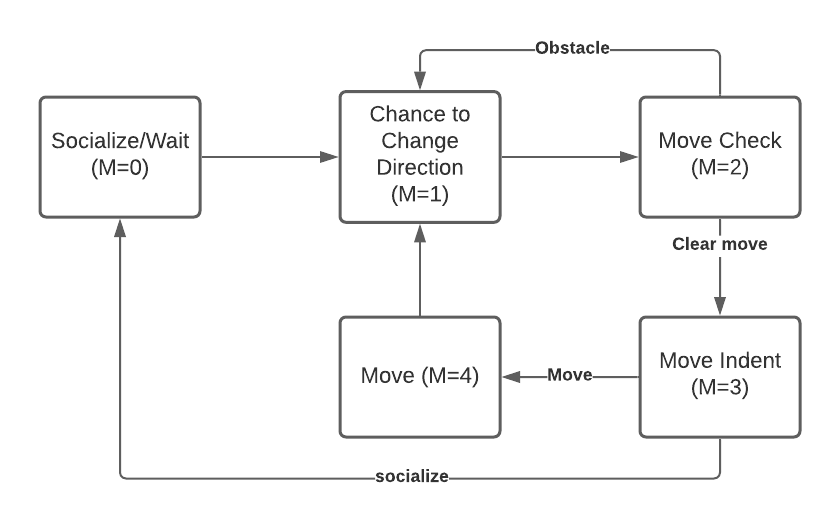
\includegraphics[scale=0.85]{../images/bee-flowchart.png}}
	\caption{The FSM or flowchart of the bee's behaviour and its transitions}
	\label{flowchart}
\end{figure}

\subsection{Formal Cell-DEVS Specification}

\begin{lstlisting}
	IDC = <X, Y, I, S, θ, N, d, δint, δext, τ, λ, D>
	X = Y = {}
	I = <η = 9, μ = 0, Px = {}, Py= {}>
	S = {s ∈ Z | 2800 <= s <= 9999}
	θ = {s, phase, f, σ} // Inertial delay
	d = { d ∈ R | 0 < d < ∞ }
	τ = {
		// Refer to encoding section for state meaning
		// TTMD - temperature, movement, direction
		// here - the neighbour (0,0), or self
		// Blank cell
		if (isBlank) { // D = 0
      		// Bee neighbours with M = 3 and direction pointing here
			if (bee moving here) {
				TT = calculateTemp()
				M = 1
				D = direction of bee moving here
				s := encode(TT, M, D)
				delay(0)
			} else { // Be not moving to this cell
				TT = calculateTemp()
				M = number of bees with M = 2 and direction pointing here
				D = 0 // Stay blank
				s := encode(TT, M, D)
				delay(0)
			}
		}
		// Bee cell
		else if (isBee) { // 1 <= D <= 8
			if (bee waiting) { // M = 0
				TT = calculateTemp()
				M = 1
				D = D
				s := encode(TT, M, D)
				// function returns in seconds, so convert to ms
				delay(waitTime() * 1000)
			} else if (bee changing direction) { // M = 1
				TT = calculateTemp()
				M = 2
				// w = random walk probability (0.1 [1])
				if (uniform(0,1) < w) {
					D = randint(1,8) // Choose new direction
				} else {
					D = D
				}
				s := encode(TT, M, D)
				delay(500) // Time to travel
			} else if () { // M = 2
			   if (noCollision) {
			   	M = 3 // Bee continues with intent
			   } else {
			   	M = 1 // Bee can't move to the cell at D
			   }
			} else if (bee move intent) { // M = 3
				TT = calculateTemp()
				// Move available and bee doesn't start socializing
				if (noCollision AND not socialize()) {
					M = 4 // Bee moves to new cell
				} else {
					M = 0 // Bee socializes
				}
				D = D
				s := encode(TT, M, D)
				delay(500) // Time to travel
			} else if (bee moving) { // M = 4
				TT = calculateTemp()
				M = 0
				D = 0 // Set to blank, bee moving out
				s := encode(TT, M, D)
				delay(0)
			}
		}
		else {
			// keep the state the same
			s := s
			delay(0)
		}
		// Functions ======
		encode(TT, M, D) = (TT * 100) + (M * 10) + D
		calculateTemp() {
			temp = 28 // Ambient temp
			for each bee in neighbour:
				temp++ // +1 degree celsius
			for each CASU in neighbour:
			    temp += CASU temp increase
			return temp
		}
		//Get wait time in seconds using function provided in [1]
		waitTime() {
			// Taken from Eq. 1 in [1]
			(power(3.09 - 0.0403 * TT,-27)/
			(power(3.09 - 0.0403 * TT,-27) + power(1.79,-27))) * 22.5 + 0.645
		}
		// Whether the bee will stop to socialize with other bees; Returns boolean
		// Stopping power parameter can be either 0.4 or 0.8
		// Bees have to be present in front of the moving bee (this)
		// Select 3 contacts infront of this bee as per [1]
		// Ex. Direction = 2 (N), neighbour bees to socialize are at NW, N, and NE
		socialize() {
			return (uniform(0,1) < 0.4) AND (bee in front of bee)
		}
		noCollision() {
			return (no bee present or moving to cell AND not wall AND not CASU)
		}
	}
\end{lstlisting}

\subsection{CD++ Definition}

The CD++ main \emph{.ma} file can be found in the listing below:
\begin{lstlisting}
	#include(encoding.inc)
	#include(cellMacros.inc)
	
	[top]
	components : bee
	
	[bee]
	type : cell
	dim : (50,50)
	delay : inertial
	defaultDelayTime : 1
	border : wrapped
	neighbors : bee(-1,-1) bee(-1,0) bee(-1,1)
	neighbors : bee(0,-1)  bee(0,0)  bee(0,1)
	neighbors : bee(1,-1)  bee(1,0)  bee(1,1)
	initialvalue : 2800
	initialCellsValue : bee.val
	localtransition : bee-rule
	
	
	[bee-rule]
	% Blank Cell Rules ===========================
	% Set temp + move indents if no bee is moving in
	rule : {(#macro(temp)) * 100 + (#macro(getBlankM)) * 10} 0 {#macro(isBlank) AND #macro(beeMoveD) = 0}
	% Move bee into the following blank cell and set M to 1
	rule : {(#macro(temp)) * 100 + 10 + #macro(beeMoveD)} 0 {#macro(isBlank) AND #macro(beeMoveD) > 0}
	% End Blank Cell Rules =======================
	
	% Bee Cell Rules =============================
	% Bee is waiting at M = 0; changing direction at M = 1; checking direction at M = 2, socializing, and broadcasting indent at M = 3, and moving to blank cell at M = 4
	rule : {(#macro(temp)) * 100 + (10 + #macro(decodeOOD))} {(#macro(waitTime)) * 1000} {#macro(isBee) AND #macro(decodeOOM) = 0}
	rule : {(#macro(temp)) * 100 + 20 + #macro(getDirection)} 0 {#macro(isBee) AND #macro(decodeOOM) = 1}
	rule : {(#macro(temp)) * 100 + (if((#macro(moveClear)),30,10)) + (#macro(decodeOOD))} 100 {#macro(isBee) AND #macro(decodeOOM) = 2}
	rule : {(#macro(temp)) * 100 + (if((#macro(moveClear)) AND (not (#macro(socialize))),40,0)) + #macro(decodeOOD)} 500 {#macro(isBee) AND #macro(decodeOOM) = 3}
	rule : {(#macro(temp)) * 100} 0 {#macro(isBee) AND #macro(decodeOOM) = 4}
	% End Bee Cell Rules =========================
	
	% Finally, stay the same if nothing was triggered
	rule : {(0,0)} 0 { t }
\end{lstlisting}

As described above in section \ref{def}, The rules of the blank and bee cells are all that is needed for the functioning of the Cell-DEVS model. The wall and CASU robot are of the same type, so they can share the same behaviour. A wall is a CASU robot that does not emit thermal energy or vice versa. This can be further supported by examining table \ref{table:per} where they share the same Direction variable value, D=9, which indicates it is an obstacle. The only difference is the CASU robot has a M of above or equal to zero. This distinction is important to make as it allows the encoding of the variables to work cleanly and stay within 4 digits.

The presented Cell-DEVS model was also attempted to be transferred to a Cadmium Cell-DEVS model to allow the representation of multiple state variables in a structure without the need for encoding and decoding. There were some complications with the installation and due to time constraints, a Cadmium version of the bee model were unable to be implemented. Although, as the authors of \cite{Stefanc2017} pointed out, the state variables needed to represent a cell in this model is very small, so encompassing all state variables into one value would save space in memory with the addition of operations for encoding and decoding values. Since the maximum state value could be 9999, then only 14 bits ($2^{14}=16384$) are needed to encode each cell space in the case of the presented model.

\section{Simulation Results}\label{results}

There are several different phases of simulations in order to validate and test the model of the bees before results can be gathered. The final phases are more concerned with the analysis of the bee behaviour and their grouping with regards to temperature, cell space size, bee concentration, and CASU robots. The figures below that display snapshots of the simulation results can be read as heat maps. The state of each cell is the encoded variables of each with temperature being in the highest position. Therefore, the baseline temperature for the environment is the ambient temperature, 28 \degree C, and anything above will change the colour of the output. The more intensive the colour the warmer the cell is. Bees in the heat map will take up 9 cells as they increase their surroundings by 1 degree. Therefore, a bee can be located in a heat map by taking the center point of the 3 by 3 squares that travel through the cell space. Walls and CASU robots will either show up as blank cells or as white. Walls and robots can also be found by observation since they are impassible cells with constant high temperatures in order to differentiate between the bees and blank cells.

\subsection{Generation of Experiments}

\begin{figure}[htbp]
	\centerline{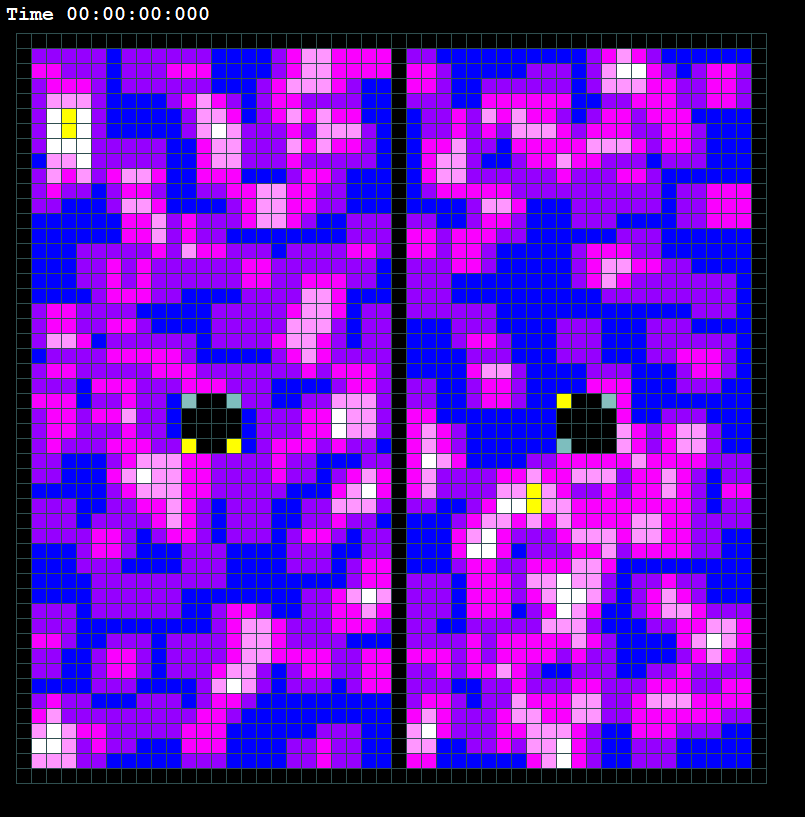
\includegraphics[scale=0.85]{../images/hive-15per-00-00-00.PNG}}
	\caption{The start of double CASU robot simulation showing robots and perimeter}
	\label{perimeter}
\end{figure}

The loading and the placement of the bees, walls, and CASU robots are done in CD++ through a \emph{.val} to update the state of specific cells. To generate the \emph{.val} files for CD++ to load, a python script was incrementally written which could randomly place a certain number of bees with respect to a set bee concentration. The listing below contains the python script to generate the \emph{.val} files. The \emph{bee\_space} variable is the bee concentration. It is the percentage of space that should be filled with bees. The script does this by multipling the bee concentration value (0.0 to 1.0) by the area of the cell space to determine the number of bees to randomly place. This isn't exact as bee could be overwritten by other randomly placed bees or be walls and CASU robots. Once all the bees are placed the CASU robots are added to the cell space. The CASU robots position is given by the \emph{casu\_robots} variable and the \emph{casu\_size} represent the area of the CASU robot. In this case the CASU robot is a 2 by 2 robot. This is done to allow the engineers to modify the surface area of the CASU robots easily. Finally, the walls are added if they are enabled. Currently, a perimeter around the cell space can be generated to bound the bees within the wrapped space. A center wall can also be added to divide the cell space into two. This can come in handy as now there are two independent simulations going on in one simulation. Figure \ref{perimeter} shows the placement of all elements described above.

\begin{lstlisting}
	import random
	import sys
	
	# Percentage of space filled with bees to study movement in different sized groups
	bee_space = 0.30
	# The placement of the casu robots(row,col)
	casu_robots = [(25,12),(25, 37)]
	casu_size = (2,2)
	casu_robot_temp = 5 # 1 < t < 9
	# Dimensions of cell space
	width = 50
	height = 50
	# Ambient temp for a single bee
	ambient_temp = 29
	
	# Whether to add walls and barrier in the center
	gen_perimeter = True
	center_wall = True
	
	for i in range(round(bee_space * width * height)):
		print("(" + str(random.randint(0,width)) + "," + 
			str(random.randint(0,height)) + ")=" + 
			str(ambient_temp) + "1" + str(random.randint(1,8)))
	
	# Generate CASU robots to control local temperature
	for robot in casu_robots:
		for row in range(casu_size[0]):
			for col in range(casu_size[1]):
				print("(" + str(robot[0] + row) + "," + 
					str(robot[1] + col) + ")=" + "50" + 
					str(casu_robot_temp) + "9")
	
	# Generate center wall
	for i in range(height):
		print("(" + str(i) + "," + str(round(width/2)) + ")=" + "9909")
	
	# # Generate walls around perimeter
	if gen_perimeter:
		for i in range(width):
			print("(0," + str(i) + ")=" + "9909")
			print("(" + str(height - 1) + "," + str(i) + ")=" + "9909")
		for i in range(height):
			print("(" + str(i) + ",0)=" + "9909")
			print("(" + str(i) + "," + str(width - 1) + ")=" + "9909")
		print("(0,0)=9909")
	else:
		print("(0,0)=2800")
	
	# Last print statement needed to avoid an error
\end{lstlisting}

\subsection{Wrapped Plane Bee Clusters}

To begin the cellular model needed to be verified to ensure that the bees were behaving correcting and no bees were being deleted or added due to collision issues. Small 10 by 10 cell spaces were constructed with bees pointing at each other to observe what would occur. After some simple bugs were ironed out, the bees random walk and socializing factors were studying to ensure the bees would always continue their random walk unless interrupted. If an interrupted occurred, from another bee only since there are no walls or CASU robots at this point, then the bee should socialize and wait for a period of time determine by their cell's temperature. During this process the socialization factor was set to 100\% in order to verify the bee could socialize. Next, the cell space was expanded and all parameters were set to their default. 25 bees were added to a cell space of 50 by 50 cells, so a bee concentration of 1\%. Even with the relatively small amount of bees in the cell space, bees were seen to cluster into groups as shown in the images in Figure \ref{initialTest}.

\begin{figure}[!tbp]
	\centering
	\begin{minipage}[b]{0.4\textwidth}
		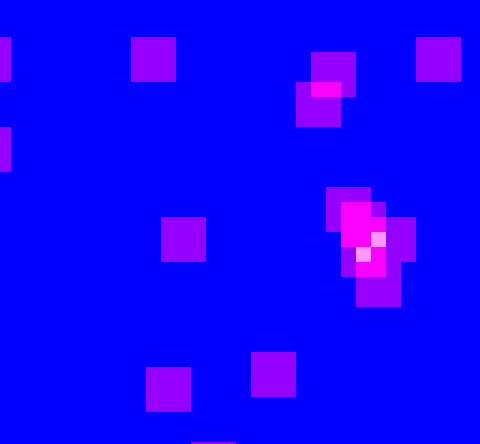
\includegraphics[width=\textwidth]{../images/cluster-example.png}
	\end{minipage}
	\hfill
	\begin{minipage}[b]{0.4\textwidth}
		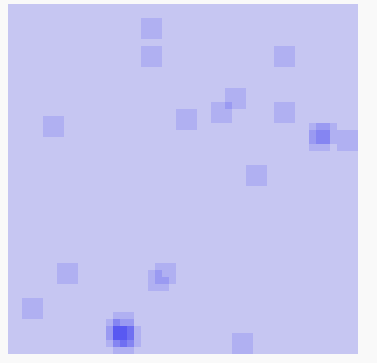
\includegraphics[width=\textwidth]{../images/cluster-2.png}
	\end{minipage}
	\caption{Small clusters forming in simulation with 25 bees in wrapped plane and 50x50 cell space}
	\label{initialTest}
\end{figure}

After the model of the bee was verified and clustering was observed to be present, the concentration of bees could be increased incrementally to simulate the effect the concentration of bees had on the clusters and groups of bees. The time length of the simulation could also be incrementally increased in the search for the system's steady state behaviour. 

\subsection{Bounded Plane Simulations}

\begin{figure}[!tbp]
	\centering
	\begin{minipage}[b]{0.4\textwidth}
		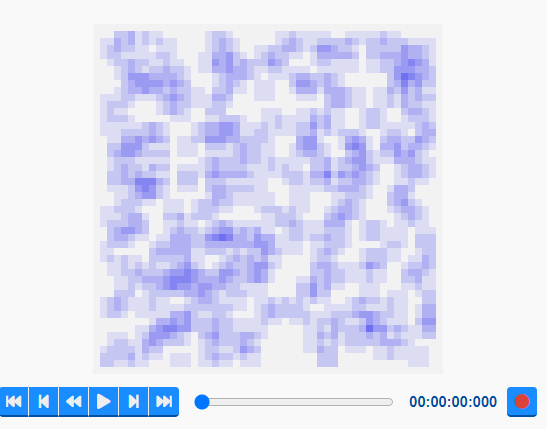
\includegraphics[width=\textwidth]{../images/hive-20per-00-00-00.PNG}
	\end{minipage}
	\hfill
	\begin{minipage}[b]{0.4\textwidth}
		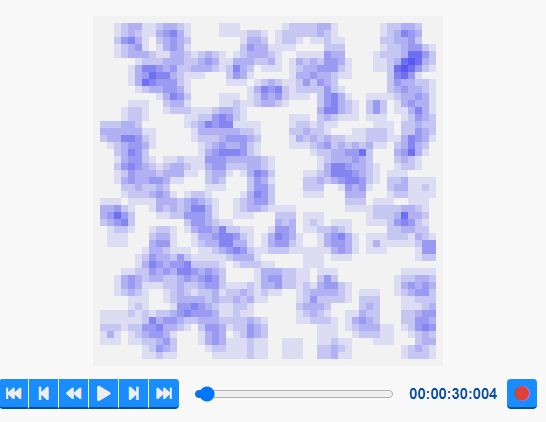
\includegraphics[width=\textwidth]{../images/hive-20per-00-30-00.PNG}
	\end{minipage}
	\caption{20\% bee concentration; Left: How the random bee placement starts; Right: 30 seconds after random start}
	\label{steady}
\end{figure}

The next series of simulations involved creating a walled perimeter, thus converting the wrapped cell space into a non-wrapped one. This could confine the bees to the cell space and ensuring they can no longer wrap around the space to simulate a close space like an artificial or actual beehive. At this point the steady state was analyzed to determine approximately how long it took for the bee movement to reach steady behaviour with varying bee concentrations. It was discovered that the bee clusters time to reach a steady state did not vary with bee concentrations. For bee concentrations of 5\%, 10\%, 15\%, 20\%, 30\%, and 50\% the steady state would be reached after about 30 seconds of real time in the simulations. This can be seen in figure \ref{steady} where the bees start with a random distribution and then 30 seconds later from the `veiny' clusters. It should be noted that steady state does not mean the clusters no longer move, but rather the size and patterns of the clusters do not change, but move in a natural looking way. In other words, the average number of bee neighbors seems to become steady.
Simulations of many length were run including 2, 5, 10, 15, 20, 45, and 60 minutes were run to determine if the bees would cluster in a large ball. This was not the case. The clusters seems to move and don't center at a specific location. The 45 and 60 minute simulations were too large ($>$30GB) to load in a visualization tool, but by using the tail tool on the CD++ \emph{.drw} files in the command line the final steps of the longer simulations were observed to still be consistent with earlier states.

\subsection{CASU Robots in Bounded Plane}

The final simulations divided the cell space into two by using a wall in the center. CASU robots were positioned in the center of each of the divided spaces as shown in figures \ref{casu-15} and \ref{casu-30-50}. To start simulations were run with the CASU robots increasing their surrounding temperatures by 1 \degree C. These simulations were expected to produce results with bee surrounding or clustering around the CASU robots, but instead the robots seem to have had little or no effect on the clusters of the bees around the robots. To attempt to resolve this, the output temperature of the CASU robots were increased to 5 \degree C and the results can be seen in figures \ref{casu-15} and \ref{casu-30-50} with varying bee concentrations. Again, it seems that the CASU robots had little or no effect of the clusters of bees across CASU temperatures and bee concentrations.

The CASU robots presented in this paper differ from the original paper, so it could explain the discrepancy between the two papers. The neighborhood of the CASU robot in the original paper used a custom neighborhood spanning a 5 by 5 area with 4 extra cells at each edge \cite{Stefanc2017}. This would increase the area that the CASU robot affects. The CASU robots in this paper were a 2 by 2 robot affecting the immediate surrounding cells. This was done to increase the surface area of the robots to provide a larger space for bees to cluster at. Some simulations were even run with the removal of the bee's local environment effect, but the bees still did not cluster around the CASU robot or even each other since there was little environment temperature increase in the system. The most likely reasons for the failure with regards to the CASU's robots are the area they affect and the bee's socializing factor is stronger than CASU's pull.

\begin{figure}[!tbp]
	\centering
	\begin{minipage}[b]{0.4\textwidth}
		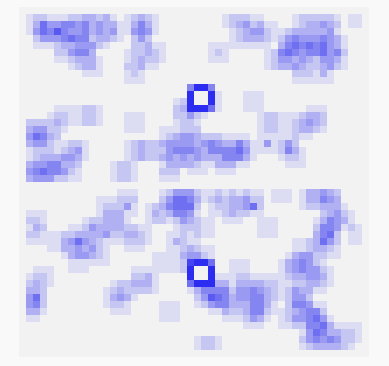
\includegraphics[width=\textwidth]{../images/hive-15per-05-00-00.PNG}
	\end{minipage}
	\hfill
	\begin{minipage}[b]{0.4\textwidth}
		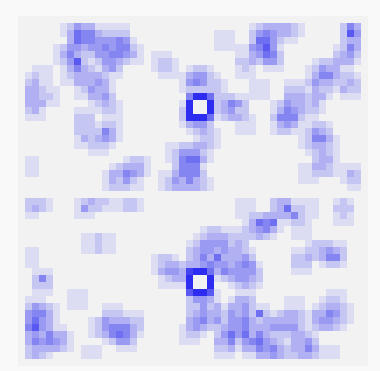
\includegraphics[width=\textwidth]{../images/hive-15per-10-00-00.PNG}
	\end{minipage}
	\caption{15\% bee concentration; 5 and 10 minutes after simulation start}
	\label{casu-15}
\end{figure}

\begin{figure}[!tbp]
	\centering
	\begin{minipage}[b]{0.4\textwidth}
		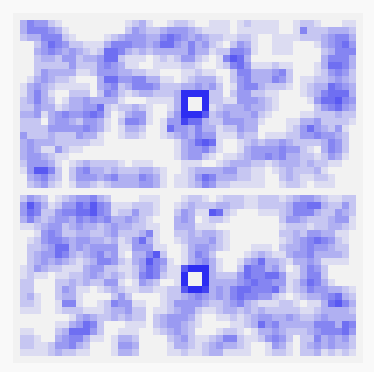
\includegraphics[width=\textwidth]{../images/hive-30per-02-00-00.PNG}
	\end{minipage}
	\hfill
	\begin{minipage}[b]{0.4\textwidth}
		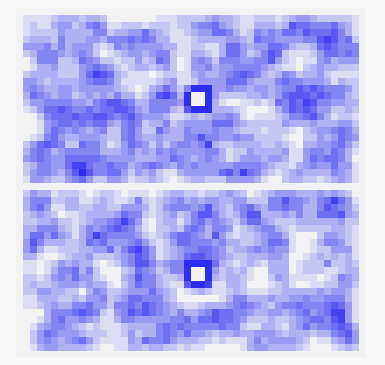
\includegraphics[width=\textwidth]{../images/hive-50per-02-00-00.PNG}
	\end{minipage}
	\caption{Left: 30\% bee concentration after 2 minutes; Right: 50\% bee concentration after 2 minutes}
	\label{casu-30-50}
\end{figure}



\section{Conclusions}\label{conclusion}

To conclude, the original paper provided a cellular automata model for the behaviour of bees with a dependency on temperature and which determined how the bees interacted with external temperature stimuli. This paper provides a proof of concept of using the bees themselves as the stimuli in an attempt to generate swarm like clusters. Figure \ref{real-bees} provide examples of a macro view of bees on a 2D honeycomb can be seen. With a quick subjective view of this paper's simulation results, it could be said that the patterns produced by the simulated bees could be similar to those in actual hives. Further analysis and verification of the model needs to be done with actual bees before an objective stance can be taken, but this work shows promising results in studying the nature of the swarm.

\begin{figure}[!tbp]
	\centering
	\begin{minipage}[b]{0.4\textwidth}
		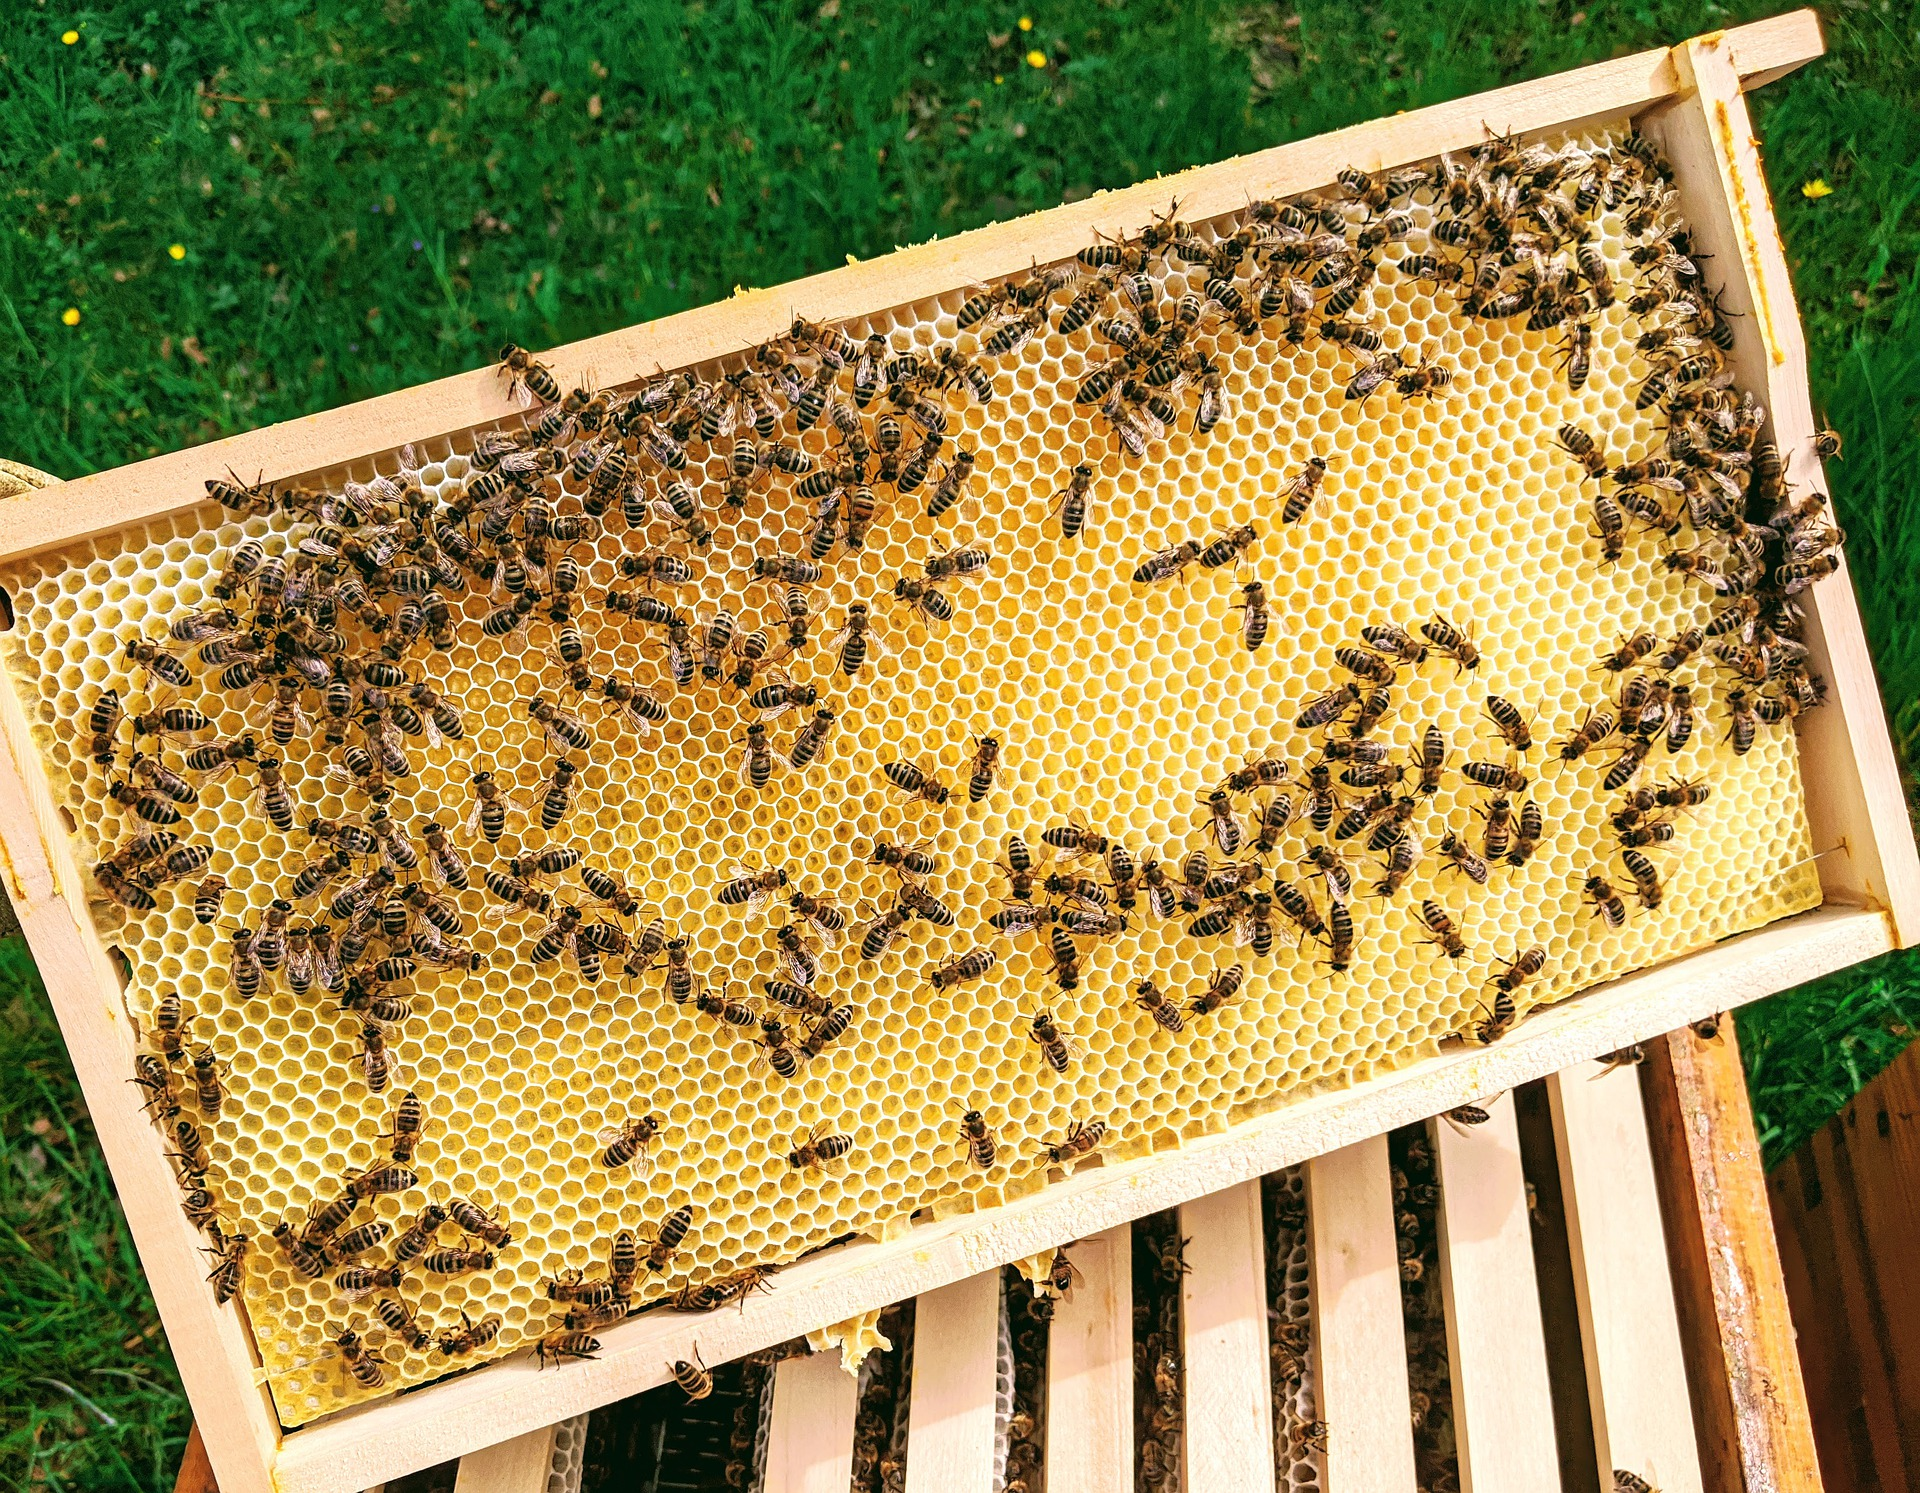
\includegraphics[width=\textwidth]{../images/bees-5491347_1920.jpg}
	\end{minipage}
	\hfill
	\begin{minipage}[b]{0.4\textwidth}
		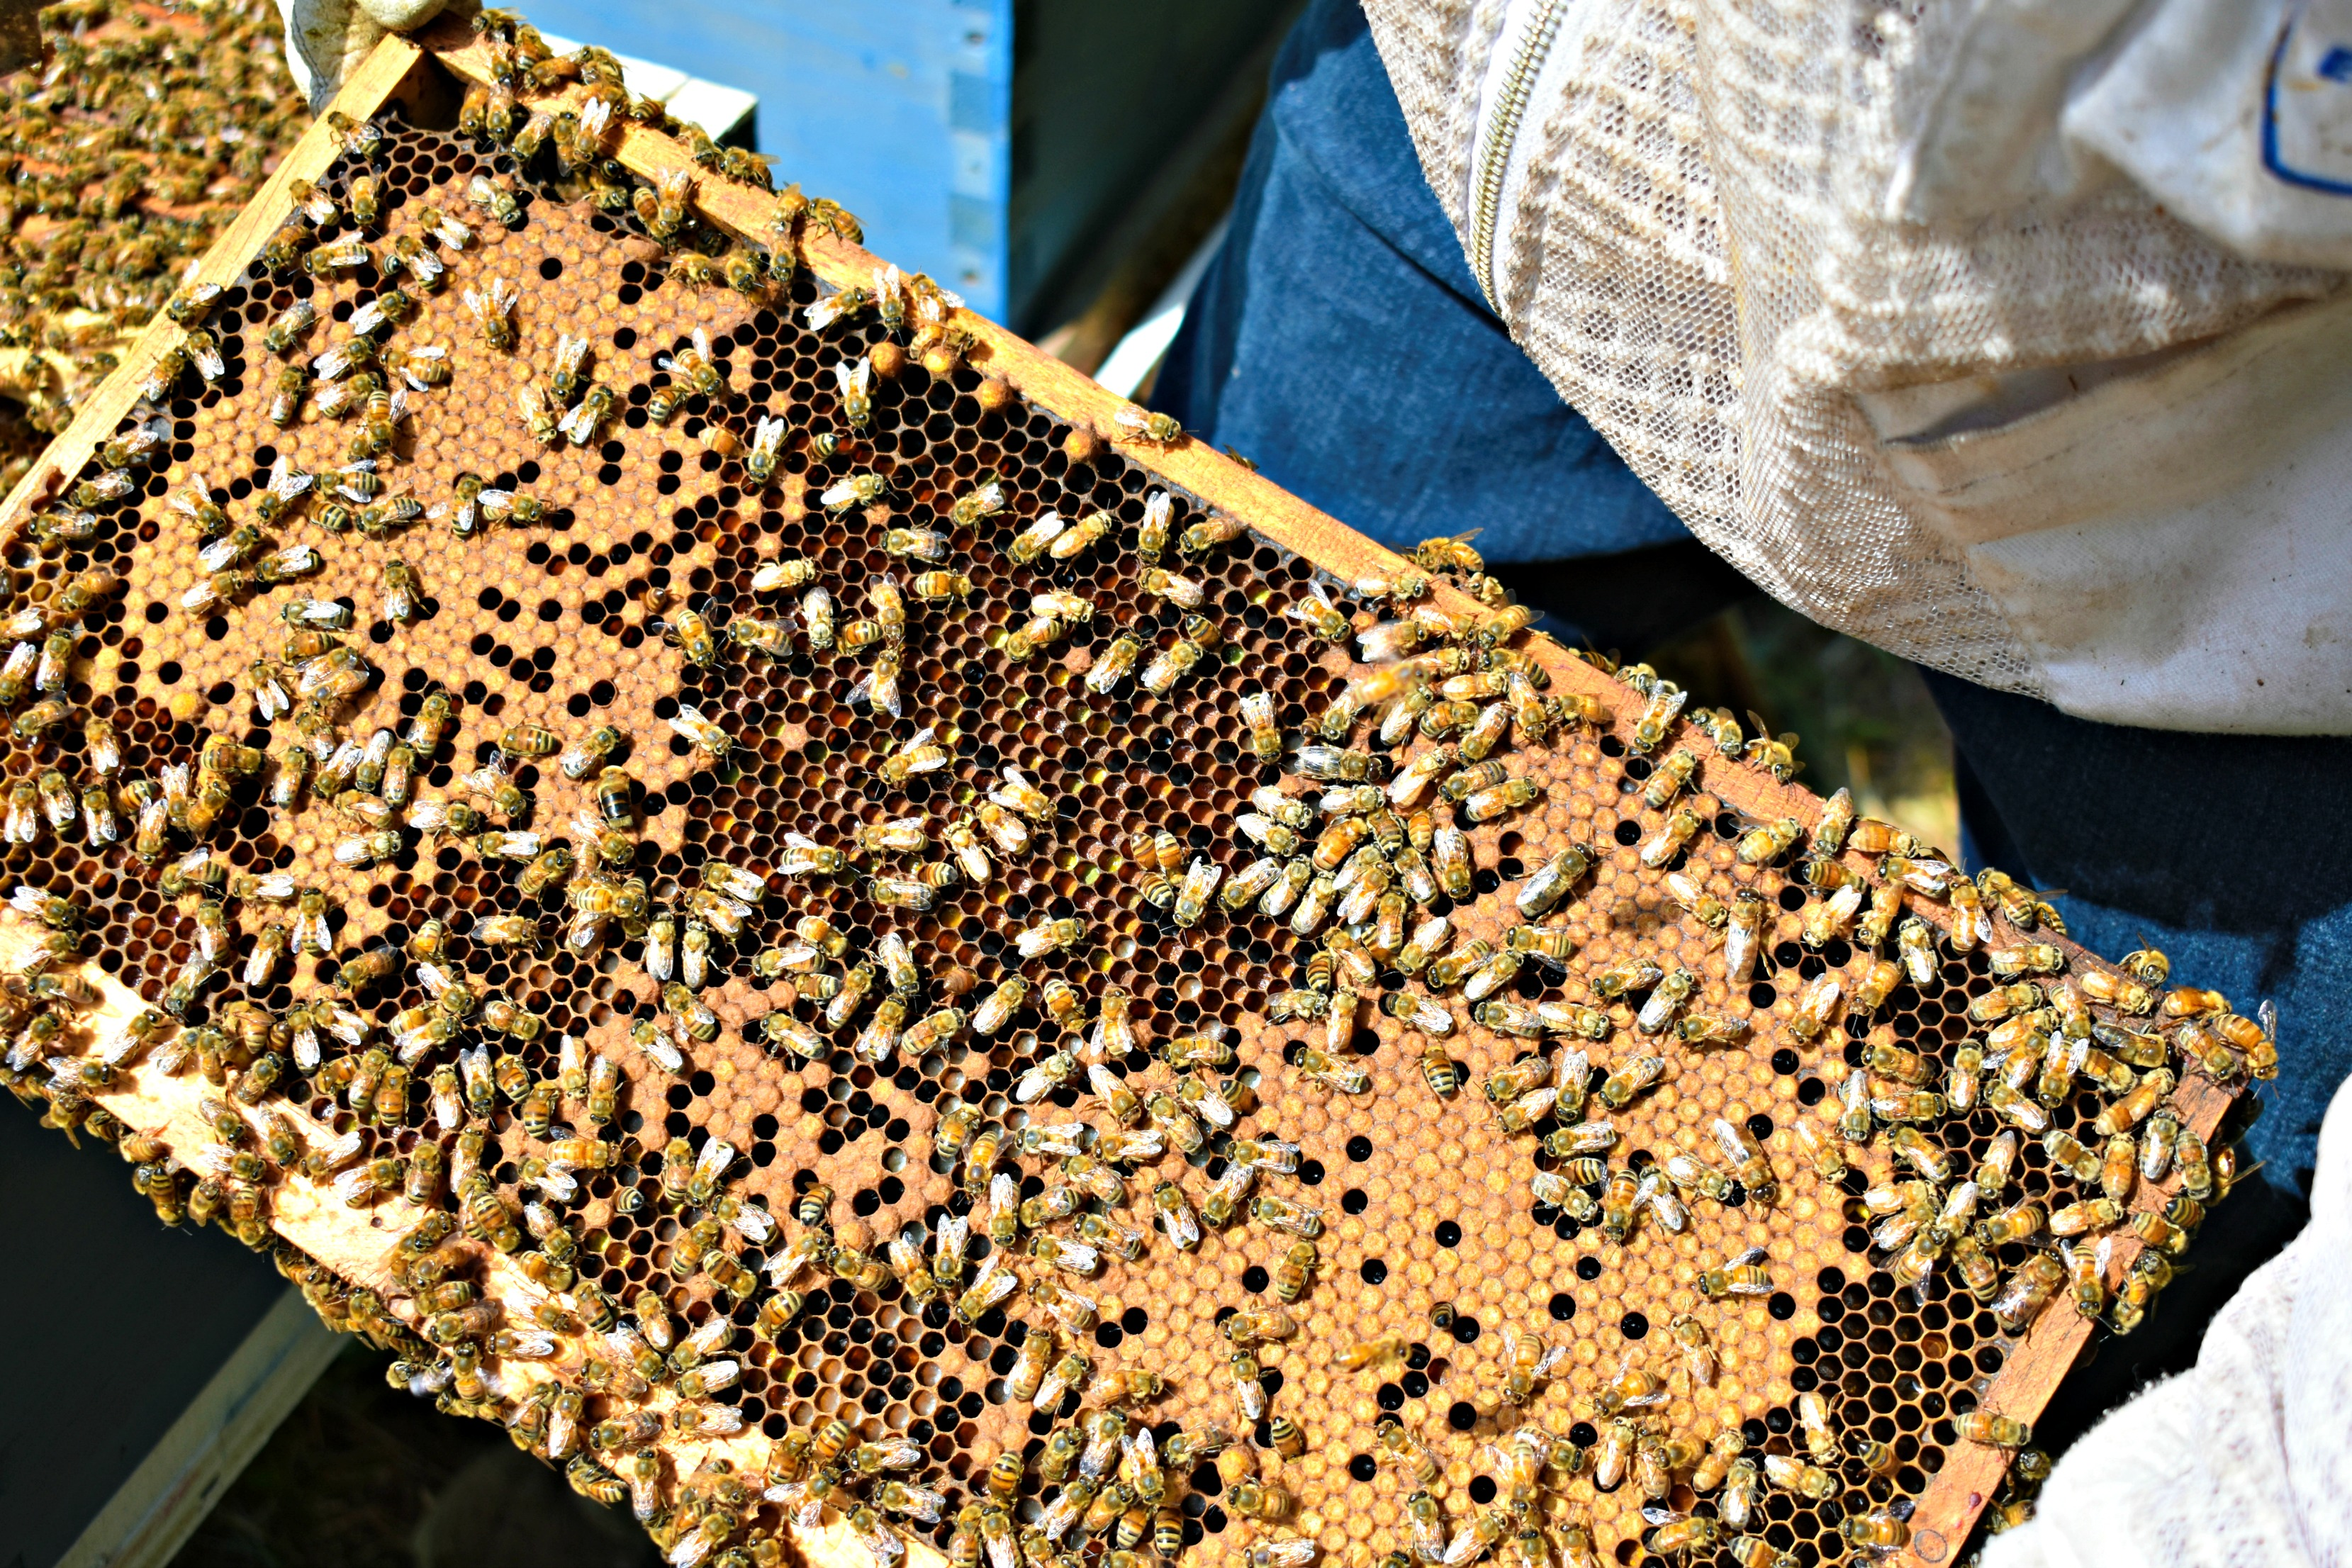
\includegraphics[width=\textwidth]{../images/freelance-sweet-on-bees-new-parasite-causing-threat-for-essential-poll_L3LYZBw.jpg}
	\end{minipage}
	\caption{Honeybees clustered across a honeycomb at different farms \cite{paetkoehler2020, Anstey2020}}
	\label{real-bees}
\end{figure}


\bibliographystyle{ieeetr}
\bibliography{Library}

\section{Appendix A}
This report may be accompanied with a series of videos which visually show the progress of the bee clusters over time in unbounded and bounded space, with and without the CASU robots. These videos may be of interest to those wishing to further studying the beehaviour of the model.

\subsection{Cell Macros}

The following listing contains some helpful macros in CD++ for calculating cell temperatures, evaluating collisions, and determining bee moves:

\begin{lstlisting}
	% This file holds macros to get temperature of the origin cell and other helper macros
	% Ambient temperature is 28 degrees celcius with each bee adding 1 degree to the area (total of 9)
	#BeginMacro(temp)
	28 + if(remainder(remainder((0,0),100), 10) >= 1 AND remainder(remainder((0,0),100), 10) <= 8, 1, 0) + 
	if(remainder(remainder((-1,-1),100), 10) >= 1 AND remainder(remainder((-1,-1),100), 10) <= 8, 1, 0) + 
	if(remainder(remainder((-1,0),100), 10) >= 1 AND remainder(remainder((-1,0),100), 10) <= 8, 1, 0) + 
	if(remainder(remainder((-1,1),100), 10) >= 1 AND remainder(remainder((-1,1),100), 10) <= 8, 1, 0) + 
	if(remainder(remainder((0,1),100), 10) >= 1 AND remainder(remainder((0,1),100), 10) <= 8, 1, 0) + 
	if(remainder(remainder((1,1),100), 10) >= 1 AND remainder(remainder((1,1),100), 10) <= 8, 1, 0) + 
	if(remainder(remainder((1,0),100), 10) >= 1 AND remainder(remainder((1,0),100), 10) <= 8, 1, 0) + 
	if(remainder(remainder((1,-1),100), 10) >= 1 AND remainder(remainder((1,-1),100), 10) <= 8, 1, 0) + 
	if(remainder(remainder((0,-1),100), 10) >= 1 AND remainder(remainder((0,-1),100), 10) <= 8, 1, 0) +
	if(remainder(remainder((-1,-1),100), 10) = 9, trunc(remainder((-1,-1),100) / 10), 0) +
	if(remainder(remainder((-1,0),100), 10) = 9, trunc(remainder((-1,0),100) / 10), 0) +
	if(remainder(remainder((-1,1),100), 10) = 9, trunc(remainder((-1,1),100) / 10), 0) +
	if(remainder(remainder((0,1),100), 10) = 9, trunc(remainder((0,1),100) / 10), 0) +
	if(remainder(remainder((1,1),100), 10) = 9, trunc(remainder((1,1),100) / 10), 0) +
	if(remainder(remainder((1,0),100), 10) = 9, trunc(remainder((1,0),100) / 10), 0) +
	if(remainder(remainder((1,-1),100), 10) = 9, trunc(remainder((1,-1),100) / 10), 0) +
	if(remainder(remainder((0,-1),100), 10) = 9, trunc(remainder((0,-1),100) / 10), 0)
	#EndMacro
	
	% Gets the bee indents from cells around blank cell
	% if a neighbour's M is above 2 and direction is at origin; there is a bee with a movement indent here
	#BeginMacro(getBlankM)
	0 + 
	if(trunc(remainder((-1,-1),100)/10) >= 1 AND remainder(remainder((-1,-1),100), 10) = 5, 1, 0) + 
	if(trunc(remainder((-1,0),100)/10)  >= 1 AND remainder(remainder((-1,0),100), 10)  = 6, 1, 0) + 
	if(trunc(remainder((-1,1),100)/10)  >= 1 AND remainder(remainder((-1,1),100), 10)  = 7, 1, 0) + 
	if(trunc(remainder((0,1),100)/10)   >= 1 AND remainder(remainder((0,1),100), 10)   = 8, 1, 0) + 
	if(trunc(remainder((1,1),100)/10)   >= 1 AND remainder(remainder((1,1),100), 10)   = 1, 1, 0) + 
	if(trunc(remainder((1,0),100)/10)   >= 1 AND remainder(remainder((1,0),100), 10)   = 2, 1, 0) + 
	if(trunc(remainder((1,-1),100)/10)  >= 1 AND remainder(remainder((1,-1),100), 10)  = 3, 1, 0) + 
	if(trunc(remainder((0,-1),100)/10)  >= 1 AND remainder(remainder((0,-1),100), 10)  = 4, 1, 0)
	#EndMacro
	
	% Return the direction (D) of the Bee entering blank cell
	% if a neighbour's M is 4 and direction is at origin; there is a bee moving here
	#BeginMacro(beeMoveD)
	0 + 
	if(trunc(remainder((-1,-1),100)/10) = 4 AND remainder(remainder((-1,-1),100), 10) = 5, 5, 0) + 
	if(trunc(remainder((-1,0),100)/10)  = 4 AND remainder(remainder((-1,0),100), 10)  = 6, 6, 0) + 
	if(trunc(remainder((-1,1),100)/10)  = 4 AND remainder(remainder((-1,1),100), 10)  = 7, 7, 0) + 
	if(trunc(remainder((0,1),100)/10)   = 4 AND remainder(remainder((0,1),100), 10)   = 8, 8, 0) + 
	if(trunc(remainder((1,1),100)/10)   = 4 AND remainder(remainder((1,1),100), 10)   = 1, 1, 0) + 
	if(trunc(remainder((1,0),100)/10)   = 4 AND remainder(remainder((1,0),100), 10)   = 2, 2, 0) + 
	if(trunc(remainder((1,-1),100)/10)  = 4 AND remainder(remainder((1,-1),100), 10)  = 3, 3, 0) + 
	if(trunc(remainder((0,-1),100)/10)  = 4 AND remainder(remainder((0,-1),100), 10)  = 4, 4, 0)
	#EndMacro
	
	% Determines whether origin cell is a bee or not by checking encoded Direction
	% Returns boolean
	#BeginMacro(isBee)
	remainder(remainder((0,0),100), 10) >= 1 AND remainder(remainder((0,0),100), 10) <= 8
	#EndMacro
	
	% Determines whether origin cell is a blank cell
	% Returns boolean
	#BeginMacro(isBlank)
	remainder(remainder((0,0),100), 10) = 0
	#EndMacro
	
	% Gets the wait time (real) for a bee, sigmoid function dependent on temperature. Values come from [1]
	#BeginMacro(waitTime)
	(power(3.09 - 0.0403 * trunc((0,0) / 100),-27)/(power(3.09 - 0.0403 * trunc((0,0) / 100),-27) + power(1.79,-27))) * 22.5 + 0.645
	#EndMacro
	
	% Chance to change direction or keep same direction
	% 10 percent chance to change direction
	#BeginMacro(getDirection)
	if(uniform(0,1) < 0.1, truncUpper(uniform(0,8)), remainder(remainder((0,0),100), 10))
	#EndMacro
	
	% Return a new direction
	#BeginMacro(changeDirection)
	truncUpper(uniform(0,8))
	#EndMacro
	
	% Whether the bee will stop to socialize with other bees; Returns boolean
	% Stopping power parameter can be either 0.4 or 0.8 and bees have to be present
	% Bees have to be present in front of the moving bee (this)
	% Select 3 contacts infront of this bee as per [1]
	% Ex. Direction = 2 (N), neighbour bees to socialize are at NW, N, and NE
	#BeginMacro(socialize)
	(uniform(0,1) < 0.8) AND (
	(remainder(remainder((0,0),100), 10) = 2 AND
	((remainder(remainder((-1,-1),100), 10) >= 1 AND remainder(remainder((-1,-1),100), 10) <= 8) OR
	(remainder(remainder((-1,0),100), 10) >= 1 AND remainder(remainder((-1,0),100), 10) <= 8) OR
	(remainder(remainder((-1,1),100), 10) >= 1 AND remainder(remainder((-1,1),100), 10) <= 8))) OR
	(remainder(remainder((0,0),100), 10) = 3 AND
	((remainder(remainder((-1,0),100), 10) >= 1 AND remainder(remainder((-1,0),100), 10) <= 8) OR
	(remainder(remainder((-1,1),100), 10) >= 1 AND remainder(remainder((-1,1),100), 10) <= 8) OR
	(remainder(remainder((0,1),100), 10) >= 1 AND remainder(remainder((0,1),100), 10) <= 8))) OR
	(remainder(remainder((0,0),100), 10) = 4 AND
	((remainder(remainder((-1,1),100), 10) >= 1 AND remainder(remainder((-1,1),100), 10) <= 8) OR
	(remainder(remainder((0,1),100), 10) >= 1 AND remainder(remainder((0,1),100), 10) <= 8) OR
	(remainder(remainder((1,1),100), 10) >= 1 AND remainder(remainder((1,1),100), 10) <= 8))) OR
	(remainder(remainder((0,0),100), 10) = 5 AND
	((remainder(remainder((0,1),100), 10) >= 1 AND remainder(remainder((0,1),100), 10) <= 8) OR
	(remainder(remainder((1,1),100), 10) >= 1 AND remainder(remainder((1,1),100), 10) <= 8) OR
	(remainder(remainder((1,0),100), 10) >= 1 AND remainder(remainder((1,0),100), 10) <= 8))) OR
	(remainder(remainder((0,0),100), 10) = 6 AND
	((remainder(remainder((1,1),100), 10) >= 1 AND remainder(remainder((1,1),100), 10) <= 8) OR
	(remainder(remainder((1,0),100), 10) >= 1 AND remainder(remainder((1,0),100), 10) <= 8) OR
	(remainder(remainder((1,-1),100), 10) >= 1 AND remainder(remainder((1,-1),100), 10) <= 8))) OR
	(remainder(remainder((0,0),100), 10) = 7 AND
	((remainder(remainder((1,0),100), 10) >= 1 AND remainder(remainder((1,0),100), 10) <= 8) OR
	(remainder(remainder((1,-1),100), 10) >= 1 AND remainder(remainder((1,-1),100), 10) <= 8) OR
	(remainder(remainder((0,-1),100), 10) >= 1 AND remainder(remainder((0,-1),100), 10) <= 8))) OR
	(remainder(remainder((0,0),100), 10) = 8 AND
	((remainder(remainder((1,-1),100), 10) >= 1 AND remainder(remainder((1,-1),100), 10) <= 8) OR
	(remainder(remainder((0,-1),100), 10) >= 1 AND remainder(remainder((0,-1),100), 10) <= 8) OR
	(remainder(remainder((-1,-1),100), 10) >= 1 AND remainder(remainder((-1,-1),100), 10) <= 8))) OR
	(remainder(remainder((0,0),100), 10) = 1 AND
	((remainder(remainder((0,-1),100), 10) >= 1 AND remainder(remainder((0,-1),100), 10) <= 8) OR
	(remainder(remainder((-1,-1),100), 10) >= 1 AND remainder(remainder((-1,-1),100), 10) <= 8) OR
	(remainder(remainder((-1,0),100), 10) >= 1 AND remainder(remainder((-1,0),100), 10) <= 8)))
	)
	#EndMacro
	
	% Checks to see if cell the bee is moving to is clear of other bees
	% M = 1 in blank cell (D = 0) if bee is moving to it, otherwise it is not clear or another bee is moving there 
	#BeginMacro(moveClear)
	(remainder(remainder((0,0),100), 10) = 1 AND trunc(remainder((-1,-1),100) / 10) = 1 AND remainder(remainder((-1,-1),100), 10) = 0) OR
	(remainder(remainder((0,0),100), 10) = 2 AND trunc(remainder((-1,0),100) / 10) = 1 AND remainder(remainder((-1,0),100), 10) = 0) OR
	(remainder(remainder((0,0),100), 10) = 3 AND trunc(remainder((-1,1),100) / 10) = 1 AND remainder(remainder((-1,1),100), 10) = 0) OR
	(remainder(remainder((0,0),100), 10) = 4 AND trunc(remainder((0,1),100) / 10) = 1 AND remainder(remainder((0,1),100), 10) = 0) OR
	(remainder(remainder((0,0),100), 10) = 5 AND trunc(remainder((1,1),100) / 10) = 1 AND remainder(remainder((1,1),100), 10) = 0) OR
	(remainder(remainder((0,0),100), 10) = 6 AND trunc(remainder((1,0),100) / 10) = 1 AND remainder(remainder((1,0),100), 10) = 0) OR
	(remainder(remainder((0,0),100), 10) = 7 AND trunc(remainder((1,-1),100) / 10) = 1 AND remainder(remainder((1,-1),100), 10) = 0) OR
	(remainder(remainder((0,0),100), 10) = 8 AND trunc(remainder((0,-1),100) / 10) = 1 AND remainder(remainder((0,-1),100), 10) = 0)
	#EndMacro
\end{lstlisting}

\end{document}
